%%%%%%%%%%%%%%%%%%%%%%%%%%%%%%%%%%%%%%%%%
% Arsclassica Article
%%%%%%%%%%%%%%%%%%%%%%%%%%%%%%%%%%%%%%%%%

%----------------------------------------------------------------------------------------
%	PACKAGES AND OTHER DOCUMENT CONFIGURATIONS
%----------------------------------------------------------------------------------------

\documentclass[
11pt, % Main document font size
letter, % Paper type, use 'letterpaper' for US Letter paper
oneside, % One page layout (no page indentation)
%twoside, % Two page layout (page indentation for binding and different headers)
%headinclude,footinclude, % Extra spacing for the header and footer
%BCOR5mm, % Binding correction
]{article} %{scrartcl}

%%%%%%%%%%%%%%%%%%%%%%%%%%%%%%%%%%%%%%%%%
% Arsclassica Article
% Structure Specification File
%
% This file has been downloaded from:
% http://www.LaTeXTemplates.com
%
% Original author:
% Lorenzo Pantieri (http://www.lorenzopantieri.net) with extensive modifications by:
% Vel (vel@latextemplates.com)
%
% License:
% CC BY-NC-SA 3.0 (http://creativecommons.org/licenses/by-nc-sa/3.0/)
%
%%%%%%%%%%%%%%%%%%%%%%%%%%%%%%%%%%%%%%%%%

%----------------------------------------------------------------------------------------
%	REQUIRED PACKAGES
%----------------------------------------------------------------------------------------

\usepackage[
nochapters, % Turn off chapters since this is an article        
beramono, % Use the Bera Mono font for monospaced text (\texttt)
eulermath,% Use the Euler font for mathematics
pdfspacing, % Makes use of pdftex’ letter spacing capabilities via the microtype package
dottedtoc % Dotted lines leading to the page numbers in the table of contents
]{classicthesis} % The layout is based on the Classic Thesis style

\usepackage{arsclassica} % Modifies the Classic Thesis package

\usepackage[T1]{fontenc} % Use 8-bit encoding that has 256 glyphs

\usepackage[utf8]{inputenc} % Required for including letters with accents

\usepackage[spanish,activeacute]{babel}

\usepackage{mathtools}

\usepackage{graphicx} % Required for including images
\graphicspath{{\main/plots/}{plots/}} % Set the default folder for images

\usepackage{enumitem} % Required for manipulating the whitespace between and within lists

\usepackage{lipsum} % Used for inserting dummy 'Lorem ipsum' text into the template

\usepackage{subfig} % Required for creating figures with multiple parts (subfigures)

\usepackage{amsmath,amssymb,amsthm} % For including math equations, theorems, symbols, etc

\usepackage{varioref} % More descriptive referencing

\usepackage{rotating}

\usepackage{array}
\newcolumntype{P}[1]{>{\centering\arraybackslash}p{#1}}
\newcolumntype{M}[1]{>{\centering\arraybackslash}m{#1}}

\newcommand{\subf}[2]{{\small\begin{tabular}[t]{@{}c@{}} #1\\#2 \end{tabular}}}

\usepackage{booktabs}

\newcommand\Tstrut{\rule{0pt}{2.6ex}}       % "top" strut
\newcommand\Bstrut{\rule[-0.9ex]{0pt}{0pt}} % "bottom" strut
\newcommand{\TBstrut}{\Tstrut\Bstrut} % top&bottom struts

\setlength{\belowcaptionskip}{-12pt}
\topmargin 2mm
\def\baselinestretch{1.1}
\textheight 8.8in \textwidth 16.3cm
\oddsidemargin -1mm
\evensidemargin -1mm

\usepackage{placeins}
%----------------------------------------------------------------------------------------
%	THEOREM STYLES
%---------------------------------------------------------------------------------------

%----------------------------------------------------------------------------------------
%	HYPERLINKS
%---------------------------------------------------------------------------------------

\hypersetup{
%draft, % Uncomment to remove all links (useful for printing in black and white)
colorlinks=true, breaklinks=true, bookmarks=true,bookmarksnumbered,
urlcolor=webbrown, linkcolor=RoyalBlue, citecolor=webgreen, % Link colors
pdftitle={}, % PDF title
pdfauthor={\textcopyright}, % PDF Author
pdfsubject={}, % PDF Subject
pdfkeywords={}, % PDF Keywords
pdfcreator={pdfLaTeX}, % PDF Creator
pdfproducer={LaTeX with hyperref and ClassicThesis} % PDF producer
} % Include the structure.tex file which specified the document structure and layout

\hyphenation{Fortran hy-phen-ation} % Specify custom hyphenation points in words with dashes where you would like hyphenation to occur, or alternatively, don't put any dashes in a word to stop hyphenation altogether

%----------------------------------------------------------------------------------------
%	TITLE AND AUTHOR(S)
%----------------------------------------------------------------------------------------

\title{\normalfont{Estudio bibliométrico del impacto académico de las publicaciones indexadas de Universidades Colombianas.}} % The article title

%\subtitle{Subtitle} % Uncomment to display a subtitle

\author{\spacedlowsmallcaps{Nelson Vanegas Arbeláez$^\dagger$}}

\date{\today.} 



\begin{document}


\renewcommand{\sectionmark}[1]{\markright{\spacedlowsmallcaps{#1}}} % The header for all pages (oneside) or for even pages (twoside)
%\renewcommand{\subsectionmark}[1]{\markright{\thesubsection~#1}} % Uncomment when using the twoside option - this modifies the header on odd pages
\lehead{\mbox{\llap{\small\thepage\kern1em\color{halfgray} \vline}\color{halfgray}\hspace{0.5em}\rightmark\hfil}} % The header style

\pagestyle{scrheadings} % Enable the headers specified in this block

%----------------------------------------------------------------------------------------
%	TABLE OF CONTENTS & LISTS OF FIGURES AND TABLES
%----------------------------------------------------------------------------------------

\maketitle % Print the title/author/date block

\setcounter{tocdepth}{2} % Set the depth of the table of contents to show sections and subsections only

\tableofcontents % Print the table of contents

%\listoffigures % Print the list of figures

%\listoftables % Print the list of tables

%----------------------------------------------------------------------------------------
%	ABSTRACT
%----------------------------------------------------------------------------------------

\section*{Abstract}

Usando fuentes abiertas de información, se  estudia el impacto académico que tienen las publicaciones académicas en las que al menos un autor declara está basado en Colombia. La revisión hecha es anónima (no se tiene en cuenta el autor) y se agrupa por institución. Debido a la complejidad se hace un análisis que solo comprende una selección de Universidades, por ello no es exhaustivo. El objetivo es tener una caracterización y una medida de la fracción de publicaciones que logran alto impacto (o son susceptibles de lograrlo). El análisis es cuantitativo y se hace una comparación con algunas instituciones latinoamericanas reconocidas. Se sacan algunas conclusiones basado en los resultados obtenidos. 



%\lipsum[1] % Dummy text

%----------------------------------------------------------------------------------------
%	AUTHOR AFFILIATIONS
%----------------------------------------------------------------------------------------

\let\thefootnote\relax\footnotetext{$\dagger$ \textit{Instituto de Física, Universidad de Antioquia, Medellín, Colombia.\\ \hphantom{$\dagger$} nelson.vanegas@udea.edu.co}}



%----------------------------------------------------------------------------------------

\newpage % Start the article content on the second page, remove this if you have a longer abstract that goes onto the second page

%----------------------------------------------------------------------------------------
%	INTRODUCTION
%----------------------------------------------------------------------------------------

\section{Introducción}

Colombia pasó de tener muy pocas publicaciones académicas, científicas o técnicas, a varios miles anuales en los últimos 20 años. Las razones son diversas pero una de ellas es el incentivo a aumentar la productividad científica propiciado por políticas públicas tales como las normas que fijan la remuneración de los profesores de las Universidades públicas. Esto se ha propagado a Universidades de carácter privado y de ahí un impulso a trabajar más en función de publicar. 

Igualmente, las medidas de aseguramiento de la calidad de la Educación Superior, específicamente las establecidas en procesos obligatorios tales como la obtención del Registro Calificado o voluntarias como la Acreditación de programas o Instituciones, han motivado a las Instituciones a promover la creación de grupos e investigación.

Numéricamente el aumento de los productos tipo artículo es enorme y se puede revisar en las plataformas de Minciencias. Sin embargo, es importante discutir otros aspectos no solo numéricos con respecto a las publicaciones hechas en Colombia al menos parcialmente. En este escrito se da una idea del impacto de estas publicaciones. Y se buscarán algunas comparaciones con latioamérica buscando aclarar e insinuar caminos hacia mejoras en el sistema de investigación y modelo colombianos. 

No es el propósito de este artículo encontrar relaciones causa efecto, es decir, concluir sobre cuál práctica o cultura académica de cual Institución es mejor en Colombia. Nuestro análisis no llega ahí, como tampoco llega a elucidar o intentar encontrar la relación de publicaciones y sus características con los \textit{rankings} de universidades. 

Este trabajo entonces busca más caracterizar nuestro trabajo académico, técnico y científico (repetimos que la creación artística queda bastante fuera de nuestro alcance). Esto esperamos que contribuya a buscar políticas acordes con nuestra realidad. 

De la misma manera el análisis que hacemos usará solo fuentes públicas de información. Es decir, bases de datos de publicaciones, artículos y producción académica que sean de libre acceso. Estas fuentes son diversas y no siempre arrojan los mismos resultados. Con lo cual es también importante decir que la conclusiones posibles tienen esa limitación como es apenas obvio: de dónde llega la información. 

Finalmente hay una motivación no menor para este estudio, buscar relaciones y medidas que permitan mejorar la productividad científica nacional. Hay una relación entre Investigación, medida en publicaciones científicas, y desarrollo, ver p.ej. \cite{ekolu}, \cite{luong} y \cite{celeste}. Y la economía colombiana, diríamos la industría y el sector productivo, necesitan de mejoras en innovación.  En 2022 Colombia obtuvo 29.2 de 100 puntos según el \textit{Global Innovation Index} de acuerdo a \cite{statista} que corresponde al puesto 63 entre las 132 economías estudiadas. Vale decir, la economía colombiana ocupa aproximadamente el puesto 44 en tamaño de economía en el mundo. 

\section{Selección de indicadores de impacto de la investigación.}

Medir el impacto de una publicación académica es bastante difícil. Publicaciones que hoy no parecen tener mucho eco en algún momento futuro pueden terminar consiguiendo mucha visibilidad internacional. Es apenas obvio que esto depende de que la publicación produzca o proponga resultados o métodos o ideas que las hagan ganar prestigio y reconocimiento. Es así como se pueden usar medidas del impacto de las citaciones logradas por el trabajo  de un autor, como el H-\textit{index}, pero con precaución.

Sin embargo, las medidas de impacto \textit{individual} al ser muy desagregadas no permiten estudiar tendencias o aspectos macro que son relevantes y en los que nos vamos a concentrar en este trabajo. En ese sentido, para este análisis vamos a usar información agregada por Institución y nuestra búsqueda será hacia artículos producidos y en los que la afiliación de al menos uno de los autores es en Colombia. Buscamos con ello visibilizar tendencias o características generales de las publicaciones colombianas y de ahí visualizar qué las diferencia.

Para este trabajo entonces seleccionamos:

\begin{enumerate}
	\item La base de datos (dataset) de producción académica de OpenAlex que es abierta al público y que contiene más de 250 millones de artículos indexados, incluyendo no solo los más conocidos títulos de revistas sino muchas fuentes de artículos en idiomas distintos al inglés y basados en lugares diversos del mundo \cite{OpenAlex}. Adicionalmente se han detectado numerosas ventajas al uso de OpenAlex con respecto a Scopus o Web of Science \cite{culbert}.
	\item Hemos usado \textit{Scimago Journal and Country Rank} \cite{scimago}, para extraer informaciópn de citaciones. En este trabajo se van a usar dos indicador de esta organización: SJR y H-\textit{index}. El primero de ellos es un indicador de \textit{prestigio} de una revista especializada. Este indicador usa las citaciones que ha tenido un artículo pero también el reconocimiento de la revista donde dicho artículo fue citado. Es decir, si un artículo que es citado en una revista de mucho reconocimiento dará lugar a un mejor indicador SJR para esa revista que una cita que proviene de una revista poco conocida. Es una transferencia de prestigio. Se trata también de información abierta y accesible por el público en general \cite{daemen} y \cite{maryland}. No toda revista que aparece en OpenAlex tiene un SJR, algunas revistas no lo tienen (algunas razones pueden ser que no son indexadas, que tienen muy poca visibilidad, algunas son subsecciones de otras publicaciones, etc.)
	\item Igualmente el índice \textit{h} fue propuesto como una medida del impacto en citas de los autores. Sin embargo, se ha ido agregando y ahora se cuenta con el Parámetro de Impacto H o H-\textit{index} que tiene en cuenta las citas en general de los artículos publicados por una revista. También puede ser consultado abiertamente y es accesible por el público \cite{western}. Casi toda revista tiene algún valor para este indicador.  
\end{enumerate}

Los indicadores mencionados pueden ser usados libremente y se cuenta con las (\textit{API -- Application programming Interface}) de forma abierta. En esta selección de indicadores se pueden escapar trabajos o artículos por múltiples razones. Sin embargo, afecta a todas las instituciones por igual así que no se espera que esta selección perjudique una institución en especial o agregue un sesgo. Sin embargo, el uso de información abierta añade el valor de volver reproducible el trabajo o ampliarlo a otras Universidades (en el anexo se dan las instrucciones, ver \S \ref{sec:anexo}.

\FloatBarrier
\begin{small}
	\begin{table}[ht!] 
		\begin{center} 
			\small %\hskip-1.2cm
			\begin{tabular}{|M{2.8cm}|M{1.5cm}|M{2.3cm}|M{1.4cm}|M{1.4cm}|M{1.4cm}|M{1.8cm}|} \hline 
				\vspace{2mm} \large \textbf{Institución}   & \vspace{2mm} \large \textbf{Multi\-campus} &\vspace{2mm} \large \textbf{Ciudad Ppal.} & \vspace{2mm} \large \textbf{Prof.} & \vspace{2mm} \large \textbf{Preg.} & \vspace{2mm} \large \textbf{Posg.} &\vspace{2mm} \large \textbf{I.D.}\\[2ex]
				\hline
				\vspace{2mm} U. Nacional de Colombia \vspace{1mm} -  UN & Sí & Bogotá DC &   2900 & 46000 & 9000  & I36243813 \\ \hline
				\vspace{2mm} 	U. de Antioquia  \vspace{1mm}-  UdeA & Sí & Medellín & 1800 & 35000 & 4000 & I3018704611 \\ \hline
				\vspace{2mm} U. de los Andes  \vspace{1mm} - Uniandes & No & Bogotá DC & 740 & 14000 & 4500 & I162096671\\ \hline
				\vspace{2mm} U. del Valle  \vspace{1mm} - Univalle & Sí & Cali & 1470 & 30000 & 2750 & I91732220 \\ \hline
				\vspace{2mm} U. Industrial de Santander  \vspace{1mm} - UIS & No & Bucaramanga & x & x & x & I115684694\\ \hline
				\vspace{2mm} U. EAFIT   \vspace{1mm}  & No & Medellín & x & x & x & I862322245 \\ \hline
				\vspace{2mm} U. Pontificia Bolivariana  \vspace{1mm} -  UPB & No & Medellín & x & x & x & I181028852\\ \hline			
				\vspace{2mm} U.  Javeriana \vspace{1mm} & No & Bogotá & x & x & x& I233745408 \\ \hline		
				\vspace{2mm} Escuela de Ingeniería de Antioquia \vspace{1mm} -  EIA & No & Medellín & x & x & x & I3018704611 \\ \hline	
				\vspace{2mm} U. Externado  \vspace{1mm} & No & Bogotá & x & x & x & I59986765 \\ \hline	
				\vspace{2mm} U. del Norte  \vspace{1mm} - Uninorte & No & Barranquilla & x & x & x & I142879360\\ \hline			
				\vspace{2mm} U. del Rosario  \vspace{1mm}  & No & Bogotá & x & x & x & I90803817 \\ \hline
				\vspace{2mm} U. de Medellín  \vspace{1mm}  & No & Medellín & x & x & x & I4210133585 \\ \hline			
				\vspace{2mm} Inst. Tecn. Metropolitano - ITM  \vspace{1mm}  & No & Medellín. & x & x & x& I4210141572\\ \hline
				\vspace{2mm} U. de Buenos Aires - UBA \vspace{1mm}  & No & Buenos Aires & x & x & x & I24354313 \\ \hline
				\vspace{2mm} Instituto Politécnico Nacional - IPN \vspace{1mm}  & No & México DF & x & x & x & I59361560 \\ \hline				
				\vspace{2mm} U. Estadual Paulista - UNESP   & Sí & Sao Pablo & x & x & x & I879563668\\ \hline
				\vspace{2mm} U. Católica de Chile  \vspace{1mm}  & No & Santiago & x & x & x & I162148367 \\ \hline
			\end{tabular}
		\end{center} 
		\caption{\normalsize \label{tab:inst} Todas las cifras redondeadas y aproximadas, tomadas de los sitios oficiales de cada institución, presentadas como referencia al tamaño de cada una.} 
	\end{table}
\end{small}
\FloatBarrier

\section{Metodología.}

Se seleccinaron universidades colombianas y en el exterior usando el criterio de incluir instituciones:
\begin{itemize}
	\item  tanto públicas como privadas.
	\item  que sean una muestra incluyendo las regiones.
	\item  que haya algunas en \textit{rankings} internacionales y otras que no.
	\item  con diferentes vocaciones, unas más inclinadas a lo técnico y otras más generales o más a las humanidades o ciencias sociales.
	\item de diferentes tamaños, medidas por número de estudiantes y profesores.
\end{itemize}

Lo anterior para tener un corte de Instituciones (en realidad todas son Instituciones de Educación Superior -- IES) que sea una muestra del sistema de educación superior. Infortundamente, debido al gran volumen de IES existentes no es viable adelantar en este punto un análisis de todas y cada una. Sin embargo, se provee el \textit{script} utilizado y se explica el software necesario para que este análisis pueda hacerse por parte de cualquiera, ver anexo \S [\ref{sec:anexo}]. 

Con respecto a las Instituciones del exterior, se seleccionaron buscando que tengan características con alguna similitud a las colombianas de la muestra. Es decir, que fueran de lationamérica y economías comparables, de tamaños también comparables (descartando algunas demasiado grandes como la Universidad Nacional Autónoma de México) y estructuras también similares (por ejemplo, con campus en varias ciudades). Finalmente se seleccionaron Universidades latinoamericanas que tienen un buen posicionamiento en términos de prestigio internacional. Usando esos criterios se seleccionaron las Universidades de la tabla [\ref{tab:inst}]. 

Usando los \textit{scripts} provistos ya mencionados, se procede a estudiar la información para cada institución a lo largo de los últimos 11 años. De este primer corte se hizo una comparación de las Universidades de la selección más significativas y se procede a hacer una comparación para esa selección en comparación con las instituciones de latinoamérica estudiadas. 

\section{Análisis.}

Un primer resultado que surge luego de revisar los datos \textit{sumados} de todas las instituciones muestra que en promedio hay un descenso en la productividad científica y académica de Colombia en los últimos años. Una posible causa podría ser la pandemia de 2020-2021, sin embargo hay que considerar que los procesos de publicación implican tiempos en ocasiones de meses entre envío de un artículo y publicación del mismo. Observando las gráficas de la figura \ref{fig:agregado}. Aunque no es el propósito de este estudio, notamos el descenso y queda la hipótesis de que sea una tendencia más extendida. 

\begin{center} \vspace{1mm}
\begin{figure}[th] \begin{center}
	\begin{tabular}{cc}
	\subf{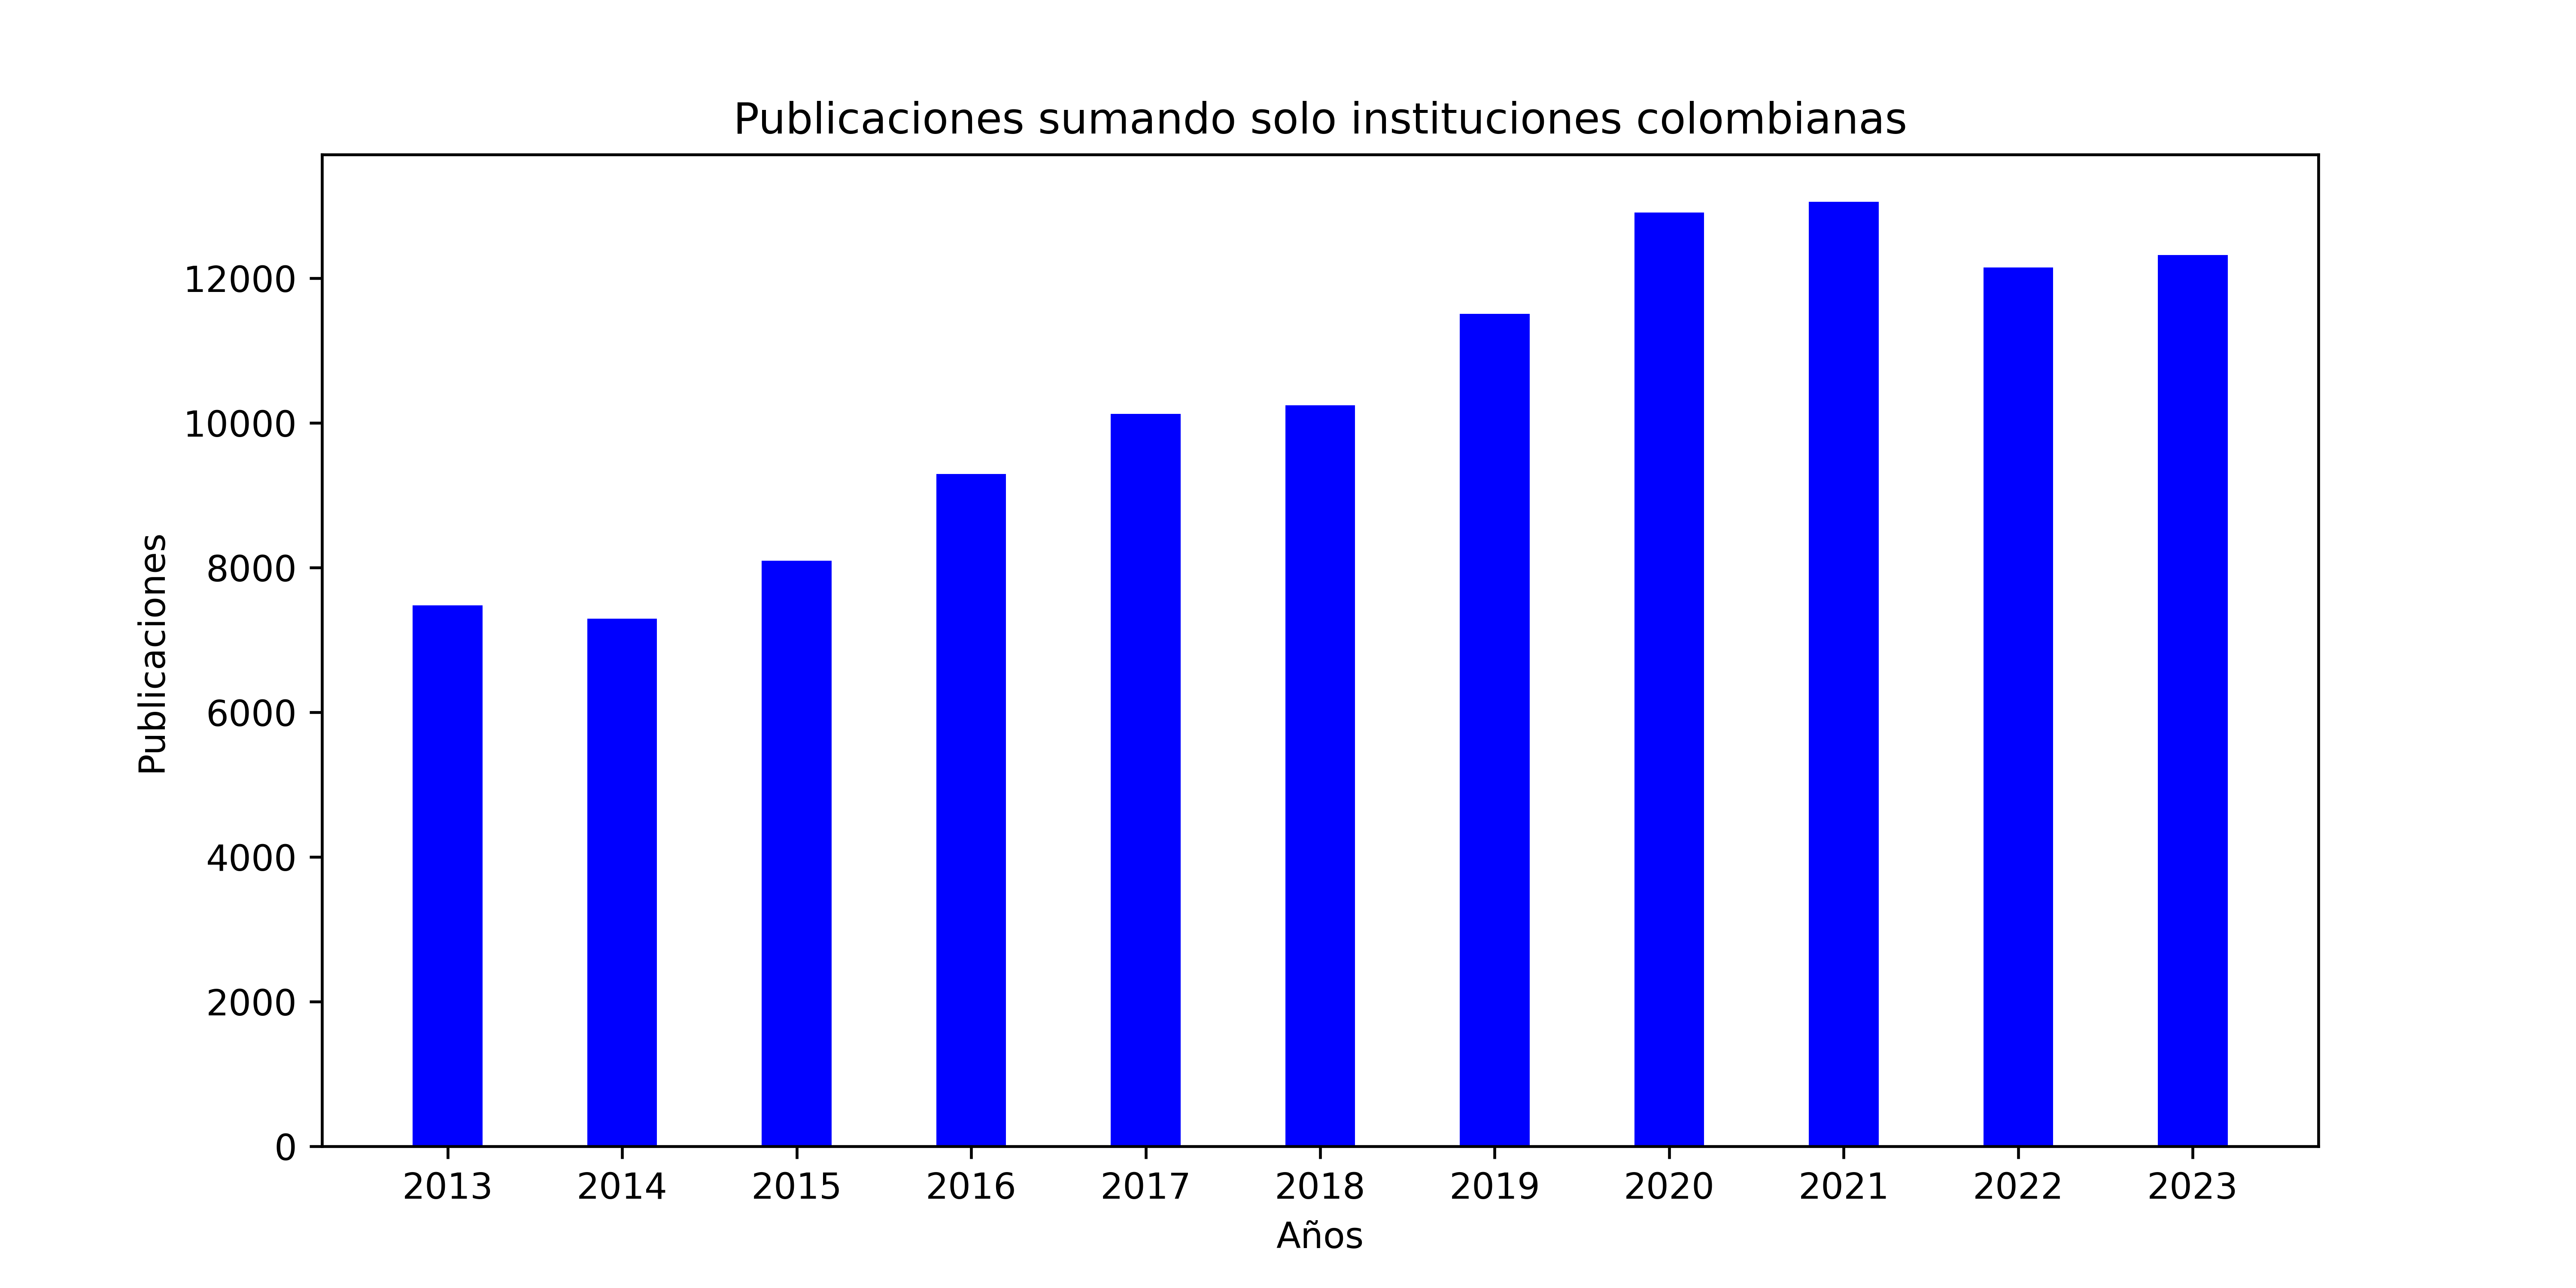
\includegraphics[width=60mm]{publicaciones_totales_colombia.png}}
	{Todas las instituciones colombianas \\ } &
	\subf{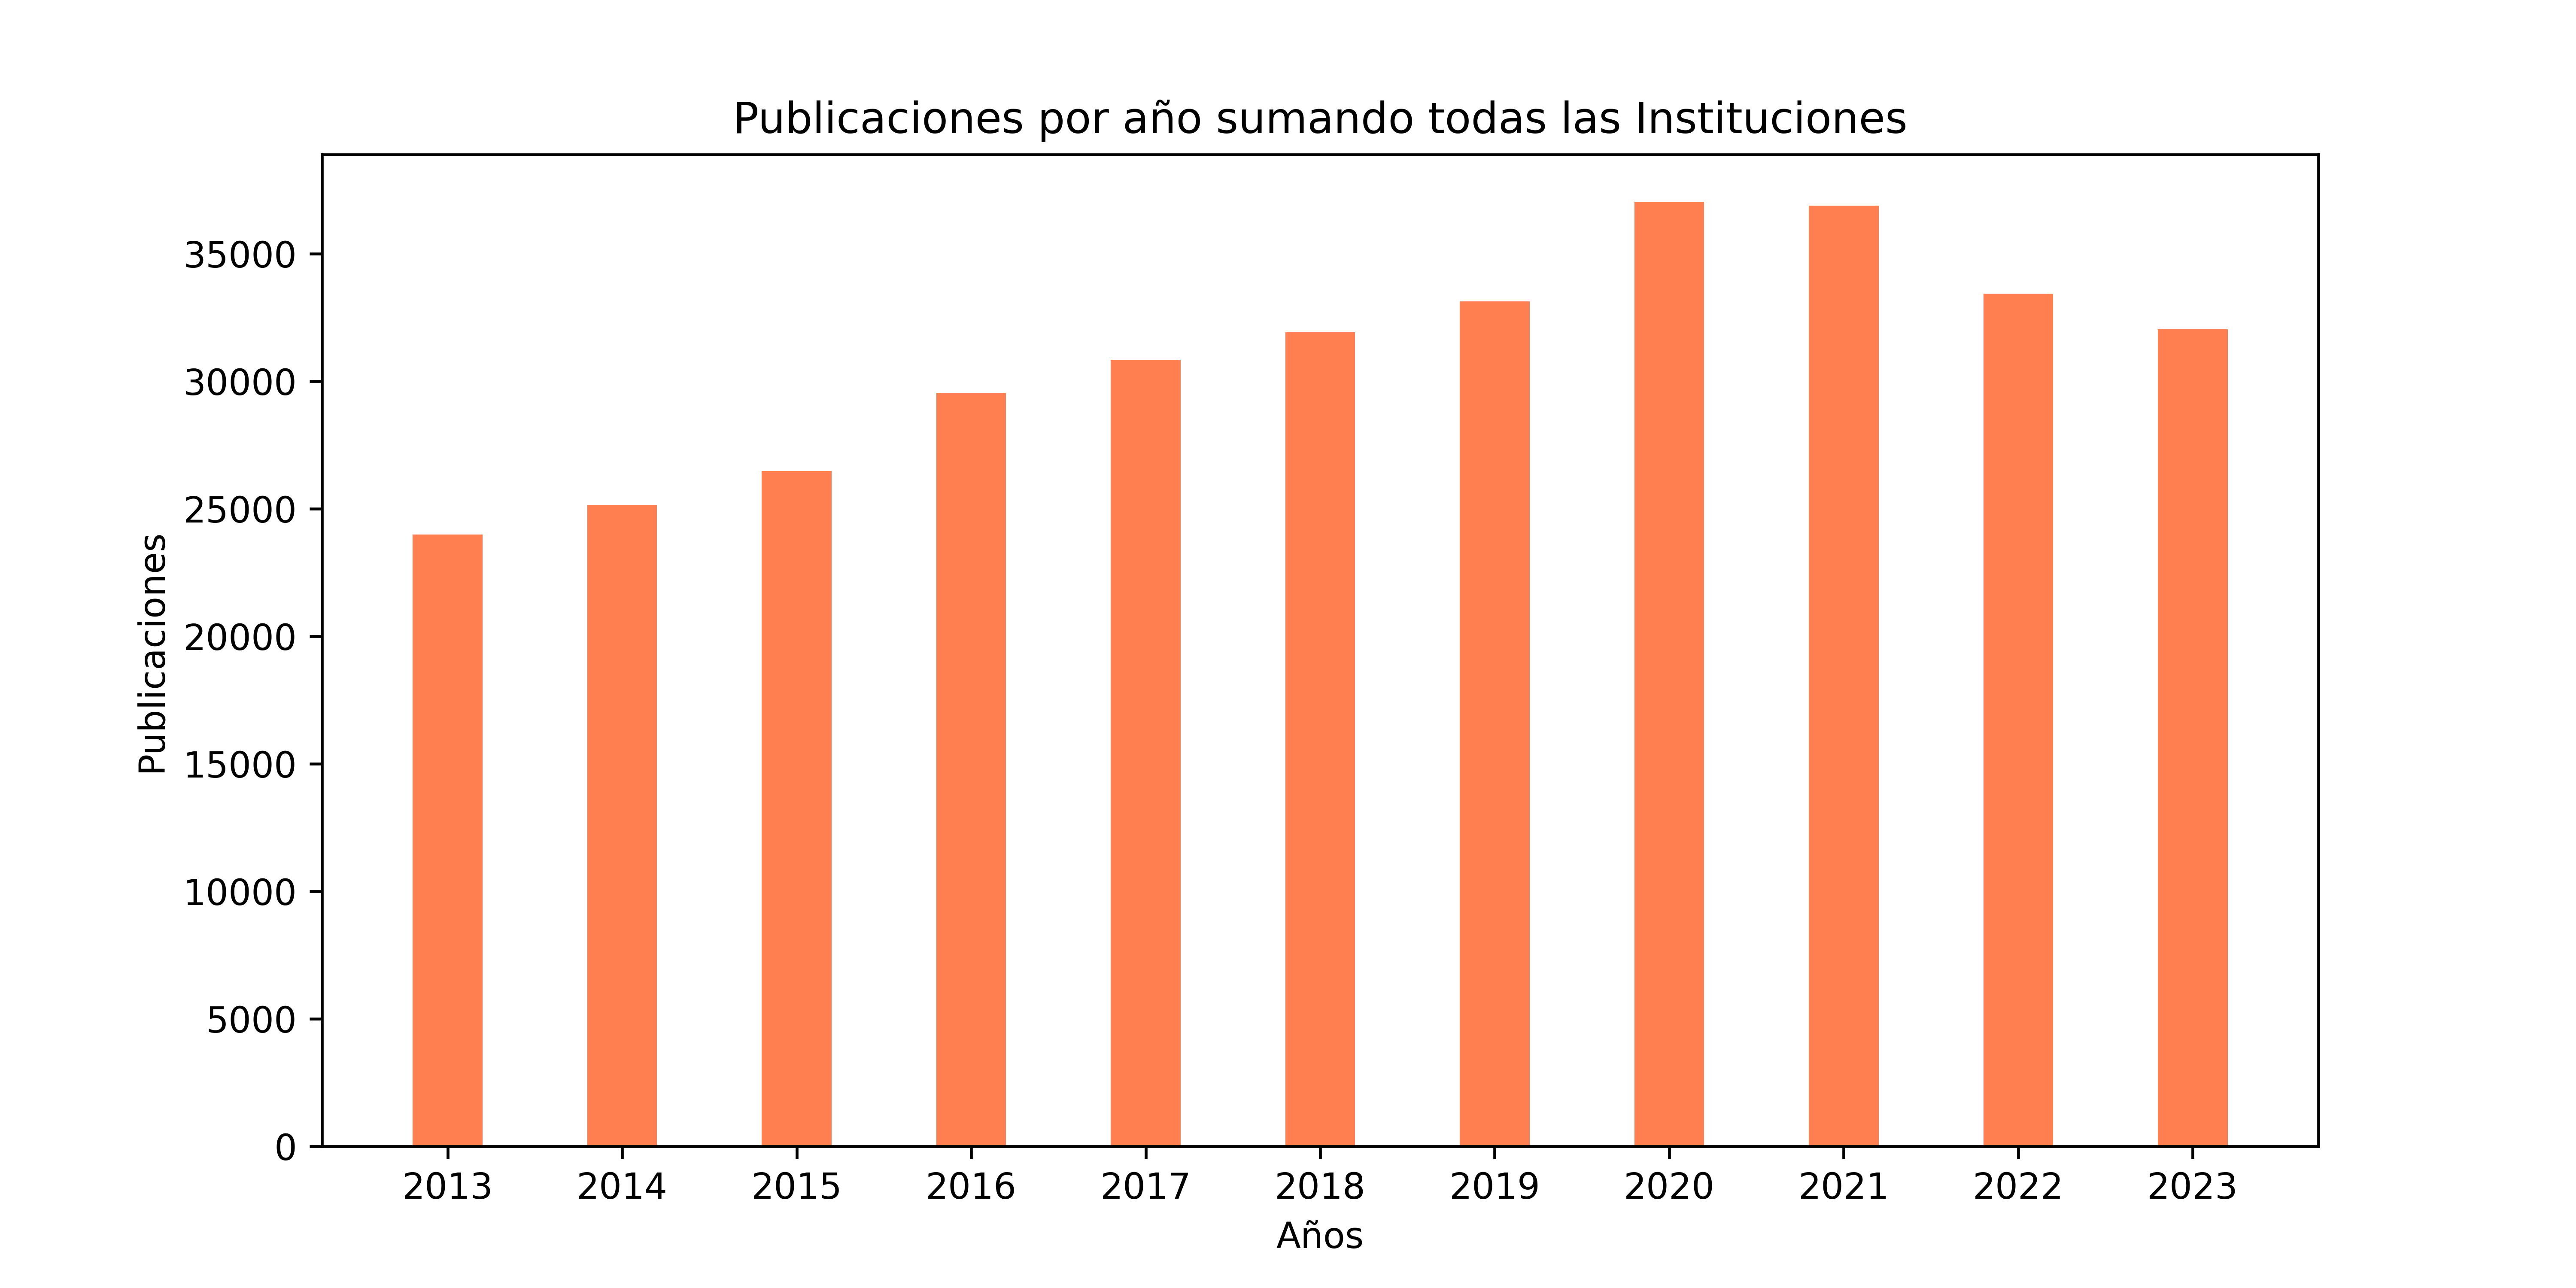
\includegraphics[width=60mm]{publicaciones_totales_todos.png}}
	{Todas las instituciones del estudio \\ }	
	\end{tabular} \caption{\label{fig:agregado} Agregado de todas las publicaciones e instituciones en el período 2013-2023.}
\end{center}
\end{figure}
\end{center} \vspace{-5mm}

Las columnas de la figura \ref{fig:agregado} deberían bajar un poco cuando se considera que en ellas se suman artículos que son producidos en colaboración entre investigadores de universidades seleccionadas y pueden estar dos veces. Una estimación de esto, por ejemplo, puede hacerse notando la cuadro \ref{tab:cern} que la U. de Antioquia comparte con la U. de los Andes, excepto pequeñas diferencias, el número de artículos publicados debido a que ambas pertenecen a la misma colaboración -- CMS. No así la U. Nacional que pertenece a la colaboración Atlas. Sin embargo, los totales de la figura \ref{fig:agregado} solo  no bajarían muy significativamente.

\begin{table}[ht]
	\begin{center} \vspace{2mm}
	\begin{tabular}{cccccc} \toprule
		\textbf{Institución} & \textbf{2019}& \textbf{2020} & \textbf{2021} & \textbf{2022} & \textbf{2023} \\ \midrule
		Uniandes & 98 & 74 & 78 & 87 & 42 \\ 
		U.Nacional &49& 89& 107 & 113 & 96 \\ 
		U .de Antioquia & 69 & 72 & 78 & 85 & 35 \\ \bottomrule
	\end{tabular}
 	\end{center} 
\caption{\small \label{tab:cern} Publicaciones de Universidades Colombianas en colaboraciones de la Organización Europea para Investigación Nuclear -- CERN.  Fuente: \url{https:\\inspirehep.net}} \vspace{2mm}
\end{table}

A paso seguido queremos ver algunas instituciones (todas están disponibles en el repositorio, pero se han seleccionado unas pocas), para establecer diferencias y características generales de los datos. En la figura \ref{fig:todos} podemos ver algunas generalidades.

La diferencia de altura entre cada columna de indicador, izquierda para JSR y derecha para H-\textit{index}, se debe a que no toda revista tiene asignado un indicador JSR. En efecto, la reputación de una revista se gana al ser citada repetidamente por artículos en revistas con JSR, lo cual requiere tiempo. En ese sentido es notorio que las publicaciones de nuestras instituciones colombianas sucede frecuentemente en publicaciones sin índice JSR (solo H). En las fuentes dadas de \textit{scimago} es claro que la probabilidad de tener citaciones aumenta con JSR. 

\begin{center} \vspace{1mm} 
	\begin{figure}[hbt!] \begin{center} \small \hskip-7mm
		\begin{tabular}{ll}
			\subf{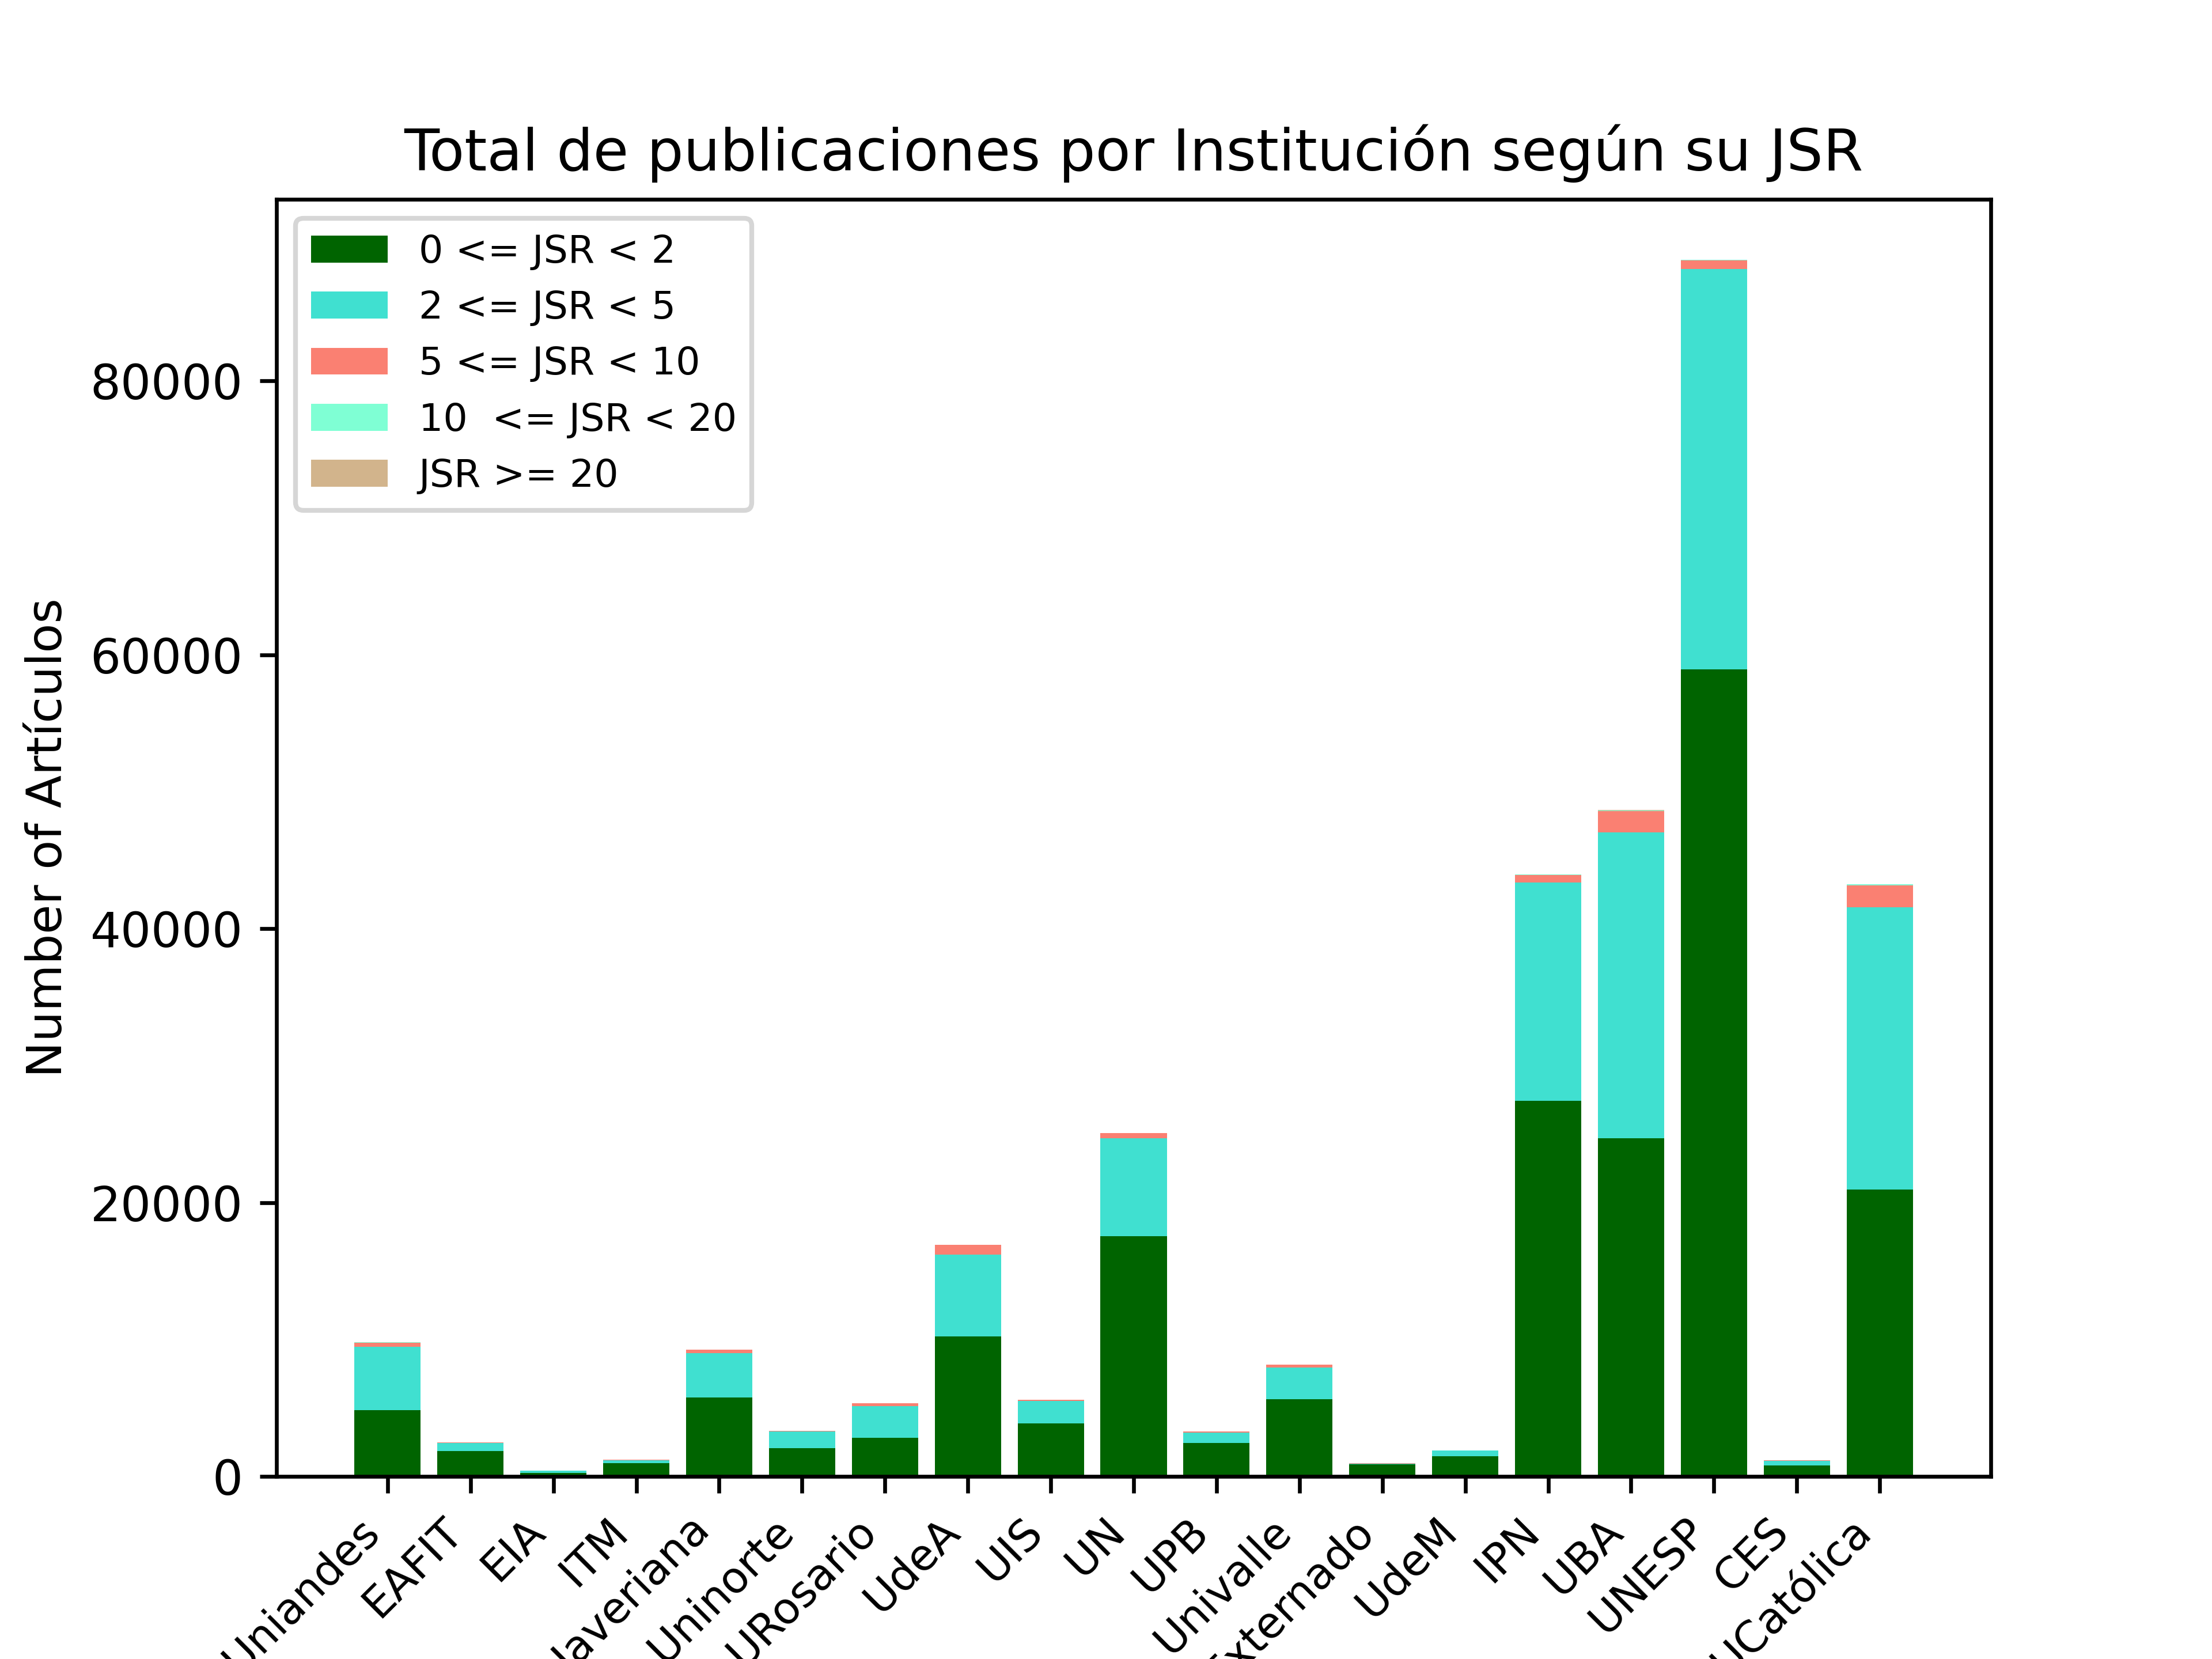
\includegraphics[width=67mm]{Inst_JSR.png}}
			{ JSR \\ } &
			\subf{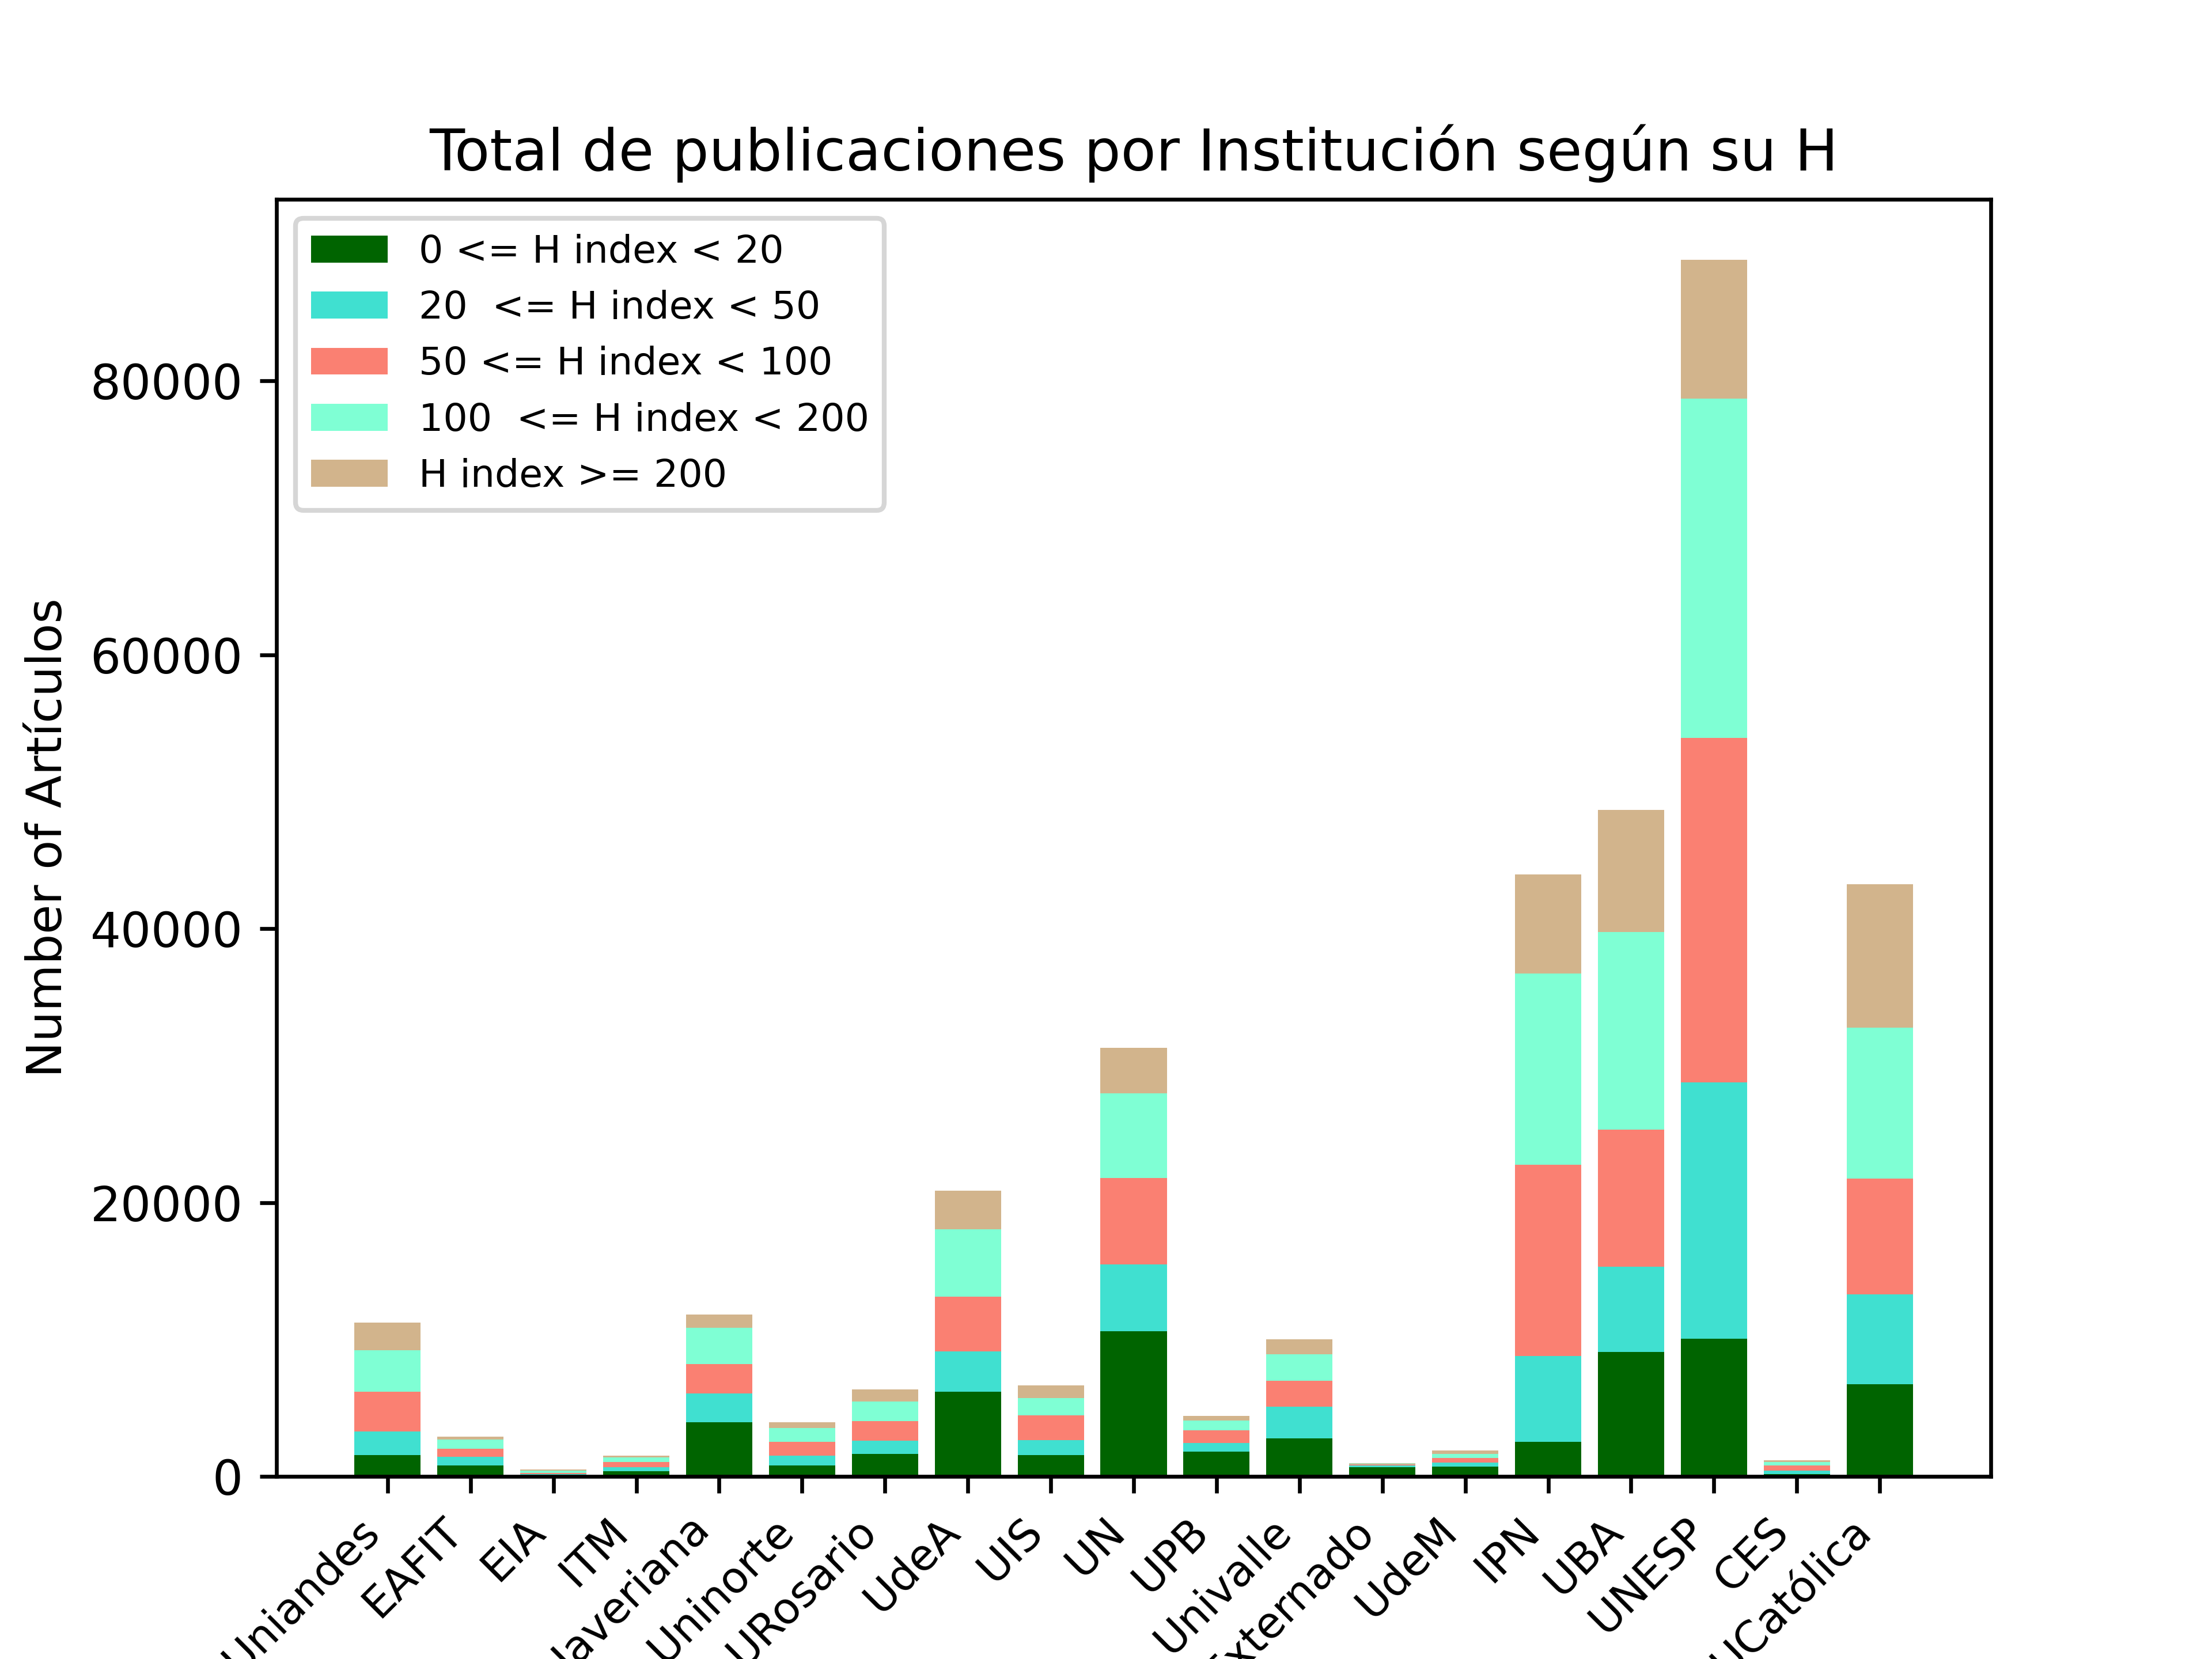
\includegraphics[width=67mm]{Inst_H.png}}
			{H-\textit{index} \\ } 
		\end{tabular} \caption{\label{fig:comparativo} Producción para las instituciones en el período 2013-2023.} \end{center}
	\end{figure} 
\end{center} %\vspace{-3mm}

Sin embargo, se observa en la misma figura que las Universidades del exterior presentadas, la diferencia entre estas columnas es indetectable. Es decir, la rata de publicación en revistas sin JSR es casi nula y en el caso colombiano puede llegar a ser notoria, dependiendo de la institución.

Lo segundo que notamos de las gráficas y datos es que las publicaciones en Colombia se centran en revistas con bajo índice JSR. Esto se nota en que en la columna de la izquierda de los gráficos predominan el primer segmento de $ 0 \leq $ JSR $ < 2$ y en el segundo $ 5 \leq $ JSR $ < 5.$ De ahí en adelante muy pocas instituciones tienen producción. Podemos decir que prácticamente toda la producción está concentrada en revistas sin JSR o menor que cinco.

Analizando la otra columna, es también claro que la producción se centra en revistas en los primeros tres rangos de H-\textit{index.} Aunque mejor distribuida y estos gráficos no hay una conclusión aparente. 

\begin{center} %\vspace{1mm}
	\begin{figure}[thb!] \begin{center}  \hskip-7mm
			\begin{tabular}{ll}
				\subf{\includegraphics[width=69mm]{UN JSR H.png}}
				{ Universidad Nacional de Colombia \\ } &
				\subf{\includegraphics[width=69mm]{Uniandes JSR H.png}}
				{Universidad de los Andes \\ } \TBstrut 	\\[10mm]
				\subf{\includegraphics[width=69mm]{UdeA JSR H.png}}
				{Universidad de Antioquia \\ } &
				\subf{\includegraphics[width=69mm]{Javeriana JSR H.png}}
				{Universidad Javeriana Bogotá\\ } \TBstrut 	\\[10mm]
				\subf{\includegraphics[width=69mm]{Univalle JSR H.png}}
				{ Universidad del Valle\\ } &
				\subf{\includegraphics[width=69mm]{Unesp JSR H.png}}
				{Universidade Estadual Paulista\\ } \TBstrut 	\\[10mm]			
				\subf{\includegraphics[width=69mm]{UCatolica JSR H.png}}
				{ Universidad Católica de Chile\\ } &
				\subf{\includegraphics[width=69mm]{IPN JSR H.png}}
				{ Instituto Politécnico Nacional\\ }
			\end{tabular} \caption{\label{fig:todos} Producción por rango del indicador H y JSR para varias instituciones en el período 2013-2023. Notar la diferencia de escala vertical en cada gŕafico.}
		\end{center}
	\end{figure}
\end{center} %\vspace{-3mm}

En términos de valores brutos de las publicaciones podemos agregar por institución las publicaciones, en la figura \ref{fig:comparativo} se muestra la suma de todo el período por institución y su distribución en rangos. Es notorio el factor de escala con las instituciones del exterior escogidas. En particular La UNESP. Sin embargo, todas tienen mucha más producción que incluso la mejor ubicada de Colombia, la Universidad Nacional. En especial, es importante comparar esta diferencia con la configuración de cada Universidad en la tabla \ref{tab:inst} que muestra número de profesores y estudiantes de pre- y posgrado. No hemos considerado pertinente retirar a la UNESP del estudio aun cuando la escala se distorsiona para mantener una institución de Brasil. 

Notando entonces las diferencias de escala y buscando centrarnos en las instituciones colombianas que más aportan en términos de publicaciones, se seleccionan las de mayor número de publicaciones para el siguiente paso.

El análisis final tiene solo se usa el H-\textit{index} toda vez que lleva más información. En la figura \ref{fig:porcentajeH} izquierda se puede identificar para cada Universidad qué tanto aporta cada rango de H al total. 

Lo que podemos ver en la misma figura es que en nuestras universidades, incluso de las de mejor producción, esta se concentra en rangos de H-\textit{index}$\leq 100.$ Que es algo que podemos verificar en la figura a la derecha. Para las instituciones colombianas en la selección la fracción promedio con rango mayor que 100 es 65.4\% mientas que en las extranjeras es 53.7\%. Si excluimos la Universidad de los andes el porcentaje de publicaciones con  H-\textit{index}$\leq 100.$ aumentaría más. 


\section{Discusión.}

Los resultados presentados pueden tener algunos errores por cuanto hemos usado bases de datos y no hemos verificado registro por registro lo encontrado. Sin embargo, los errores en general son aleatorios y afectan a cada institución por igual. Pueden deberse a artículos que deletrean mal el nombre de la institución o errores similares. Dado que los autores generalmente necesitan mostrar esta producción como propia, típicamente esto se corrige. 

Igualmente hay un error al contabilizar dos veces las colaboraciones. Las Universidades citan como propia los artículos de sus investigadores y por ende un mismo artículo puede ser contado dos veces (esto afecta especialmente los agregados nacionales). Sin embargo, aun en los casos de colaboraciones prolíficas como las del CERN, el número no es en suma muy importante para el total. 

\FloatBarrier
\begin{center} \vspace{1mm}
	\begin{figure}[hbt!] \begin{center} \small \hskip-7mm
			\begin{tabular}{ll}
				\subf{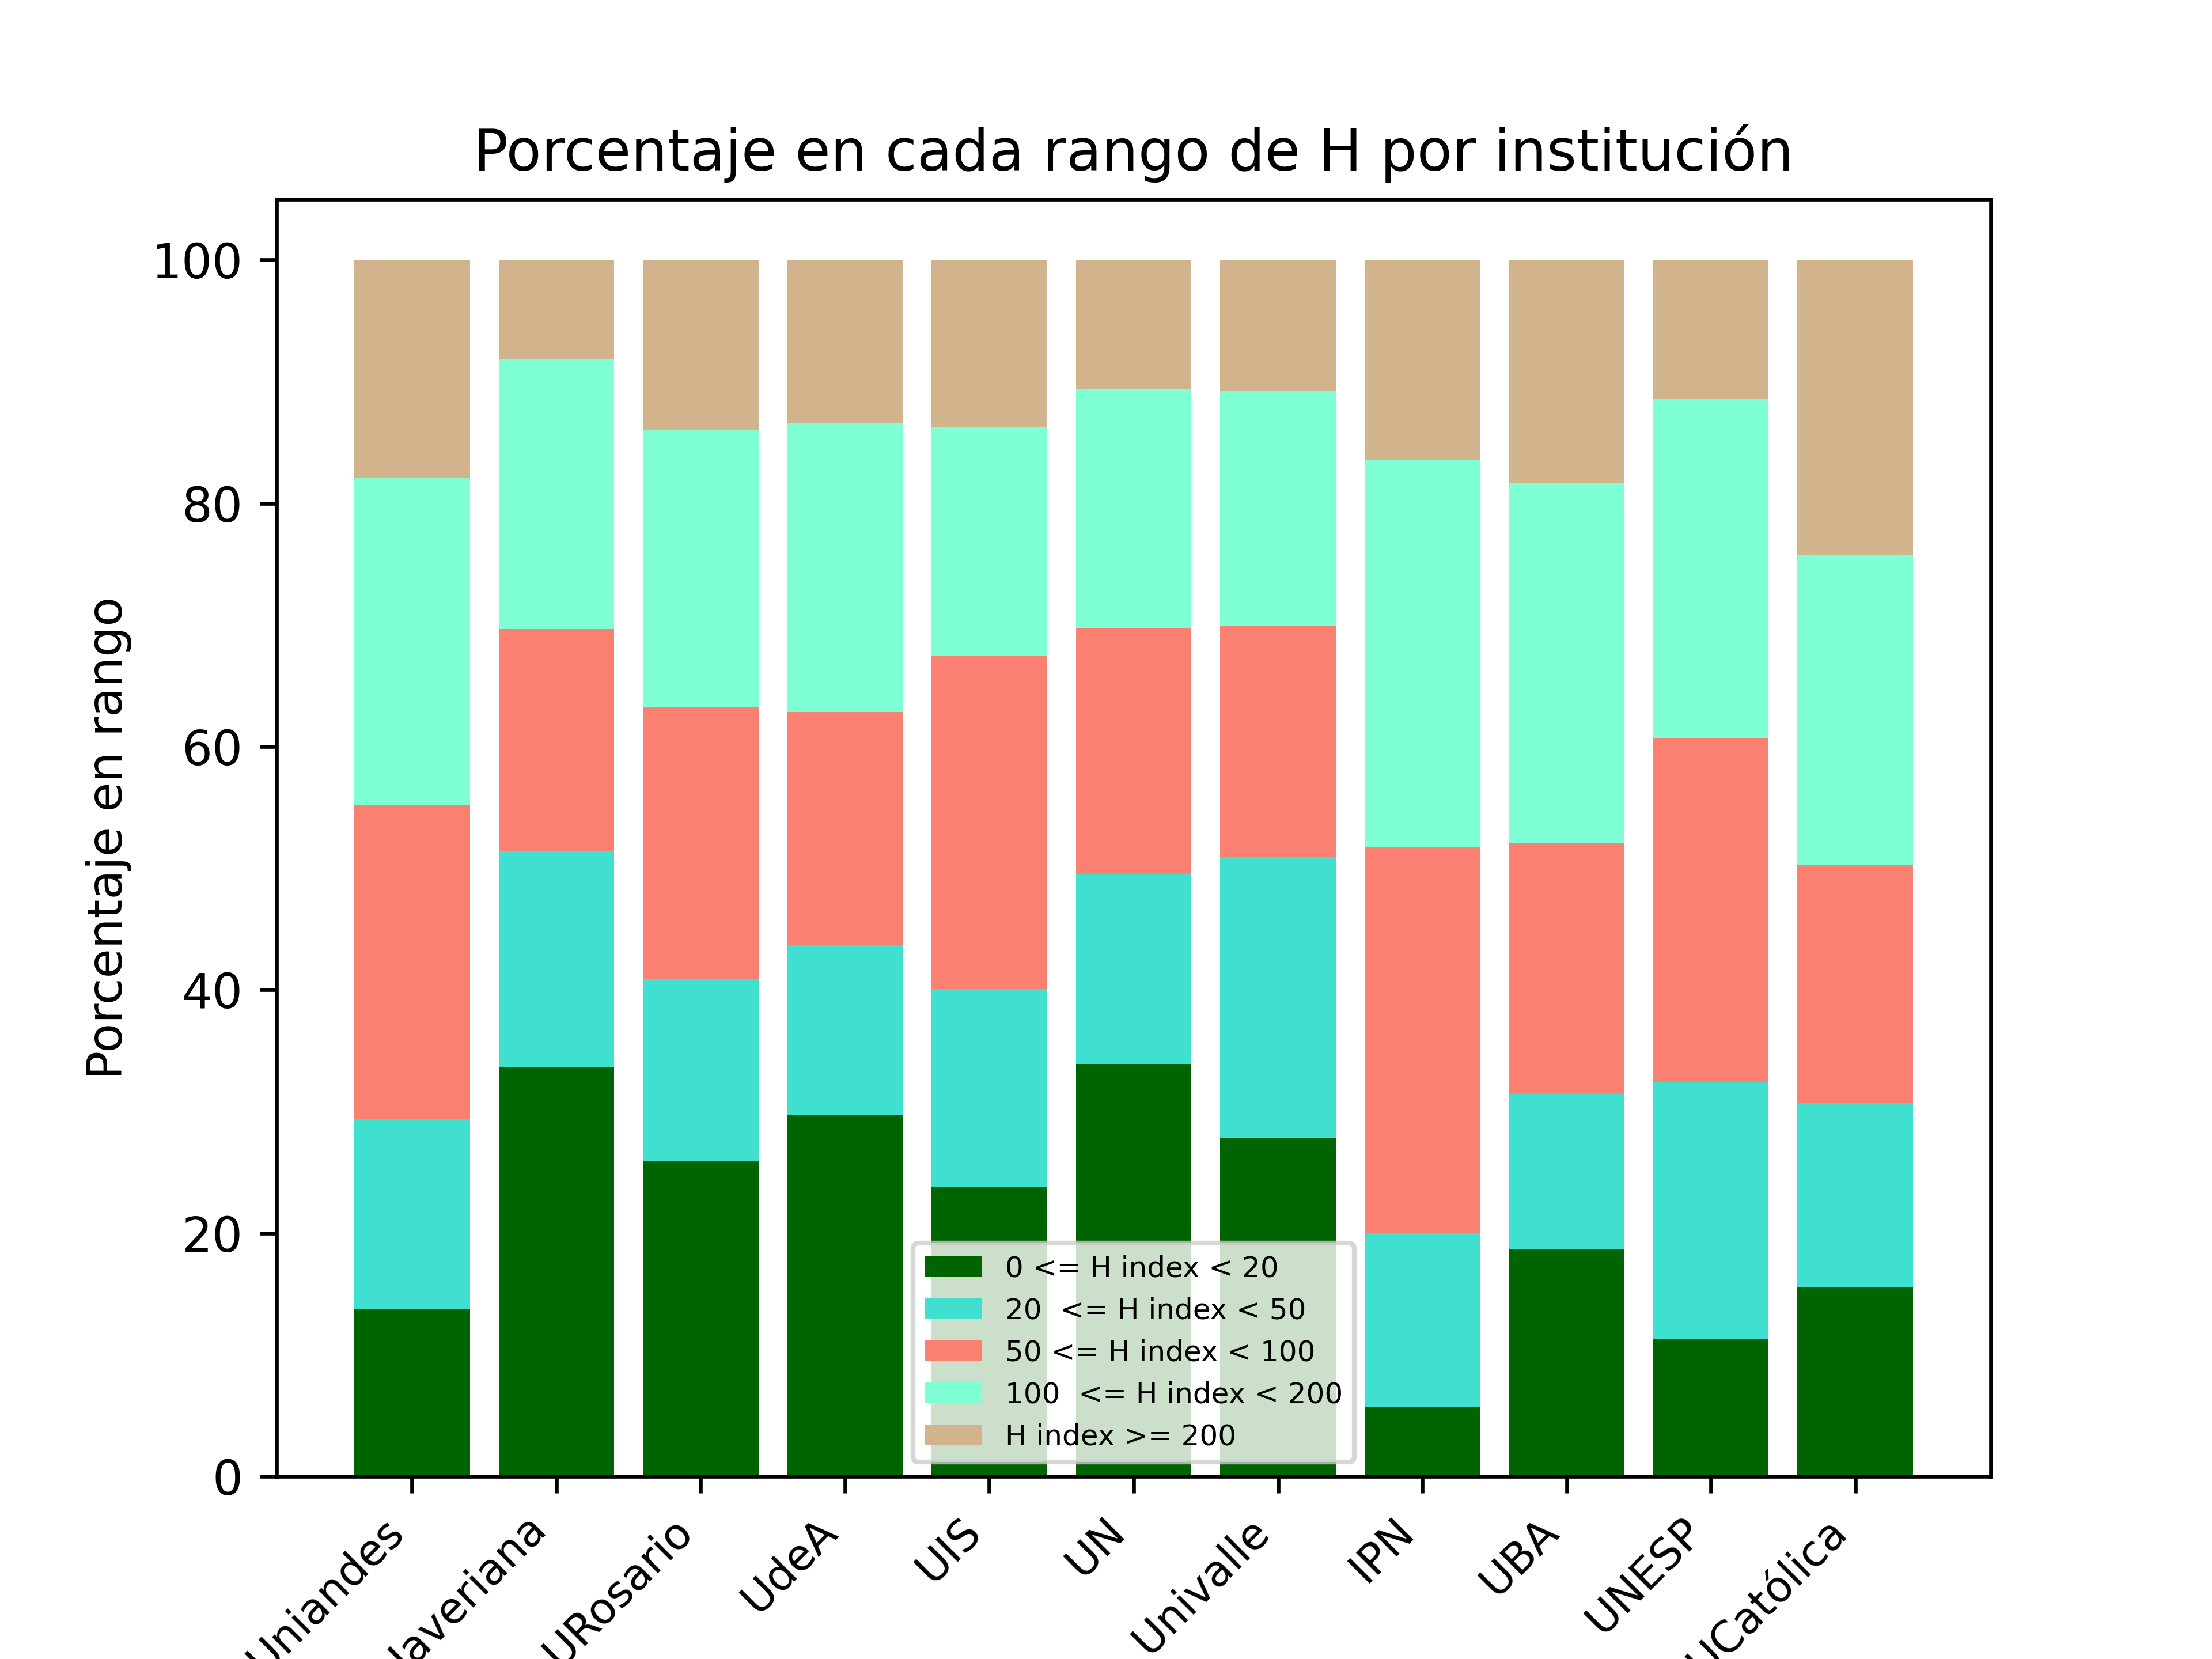
\includegraphics[width=67mm]{Porcentajes_seleccion_rango_H.png}}
				{Fracción en cada rango de H-\textit{index}\\ } &
				\subf{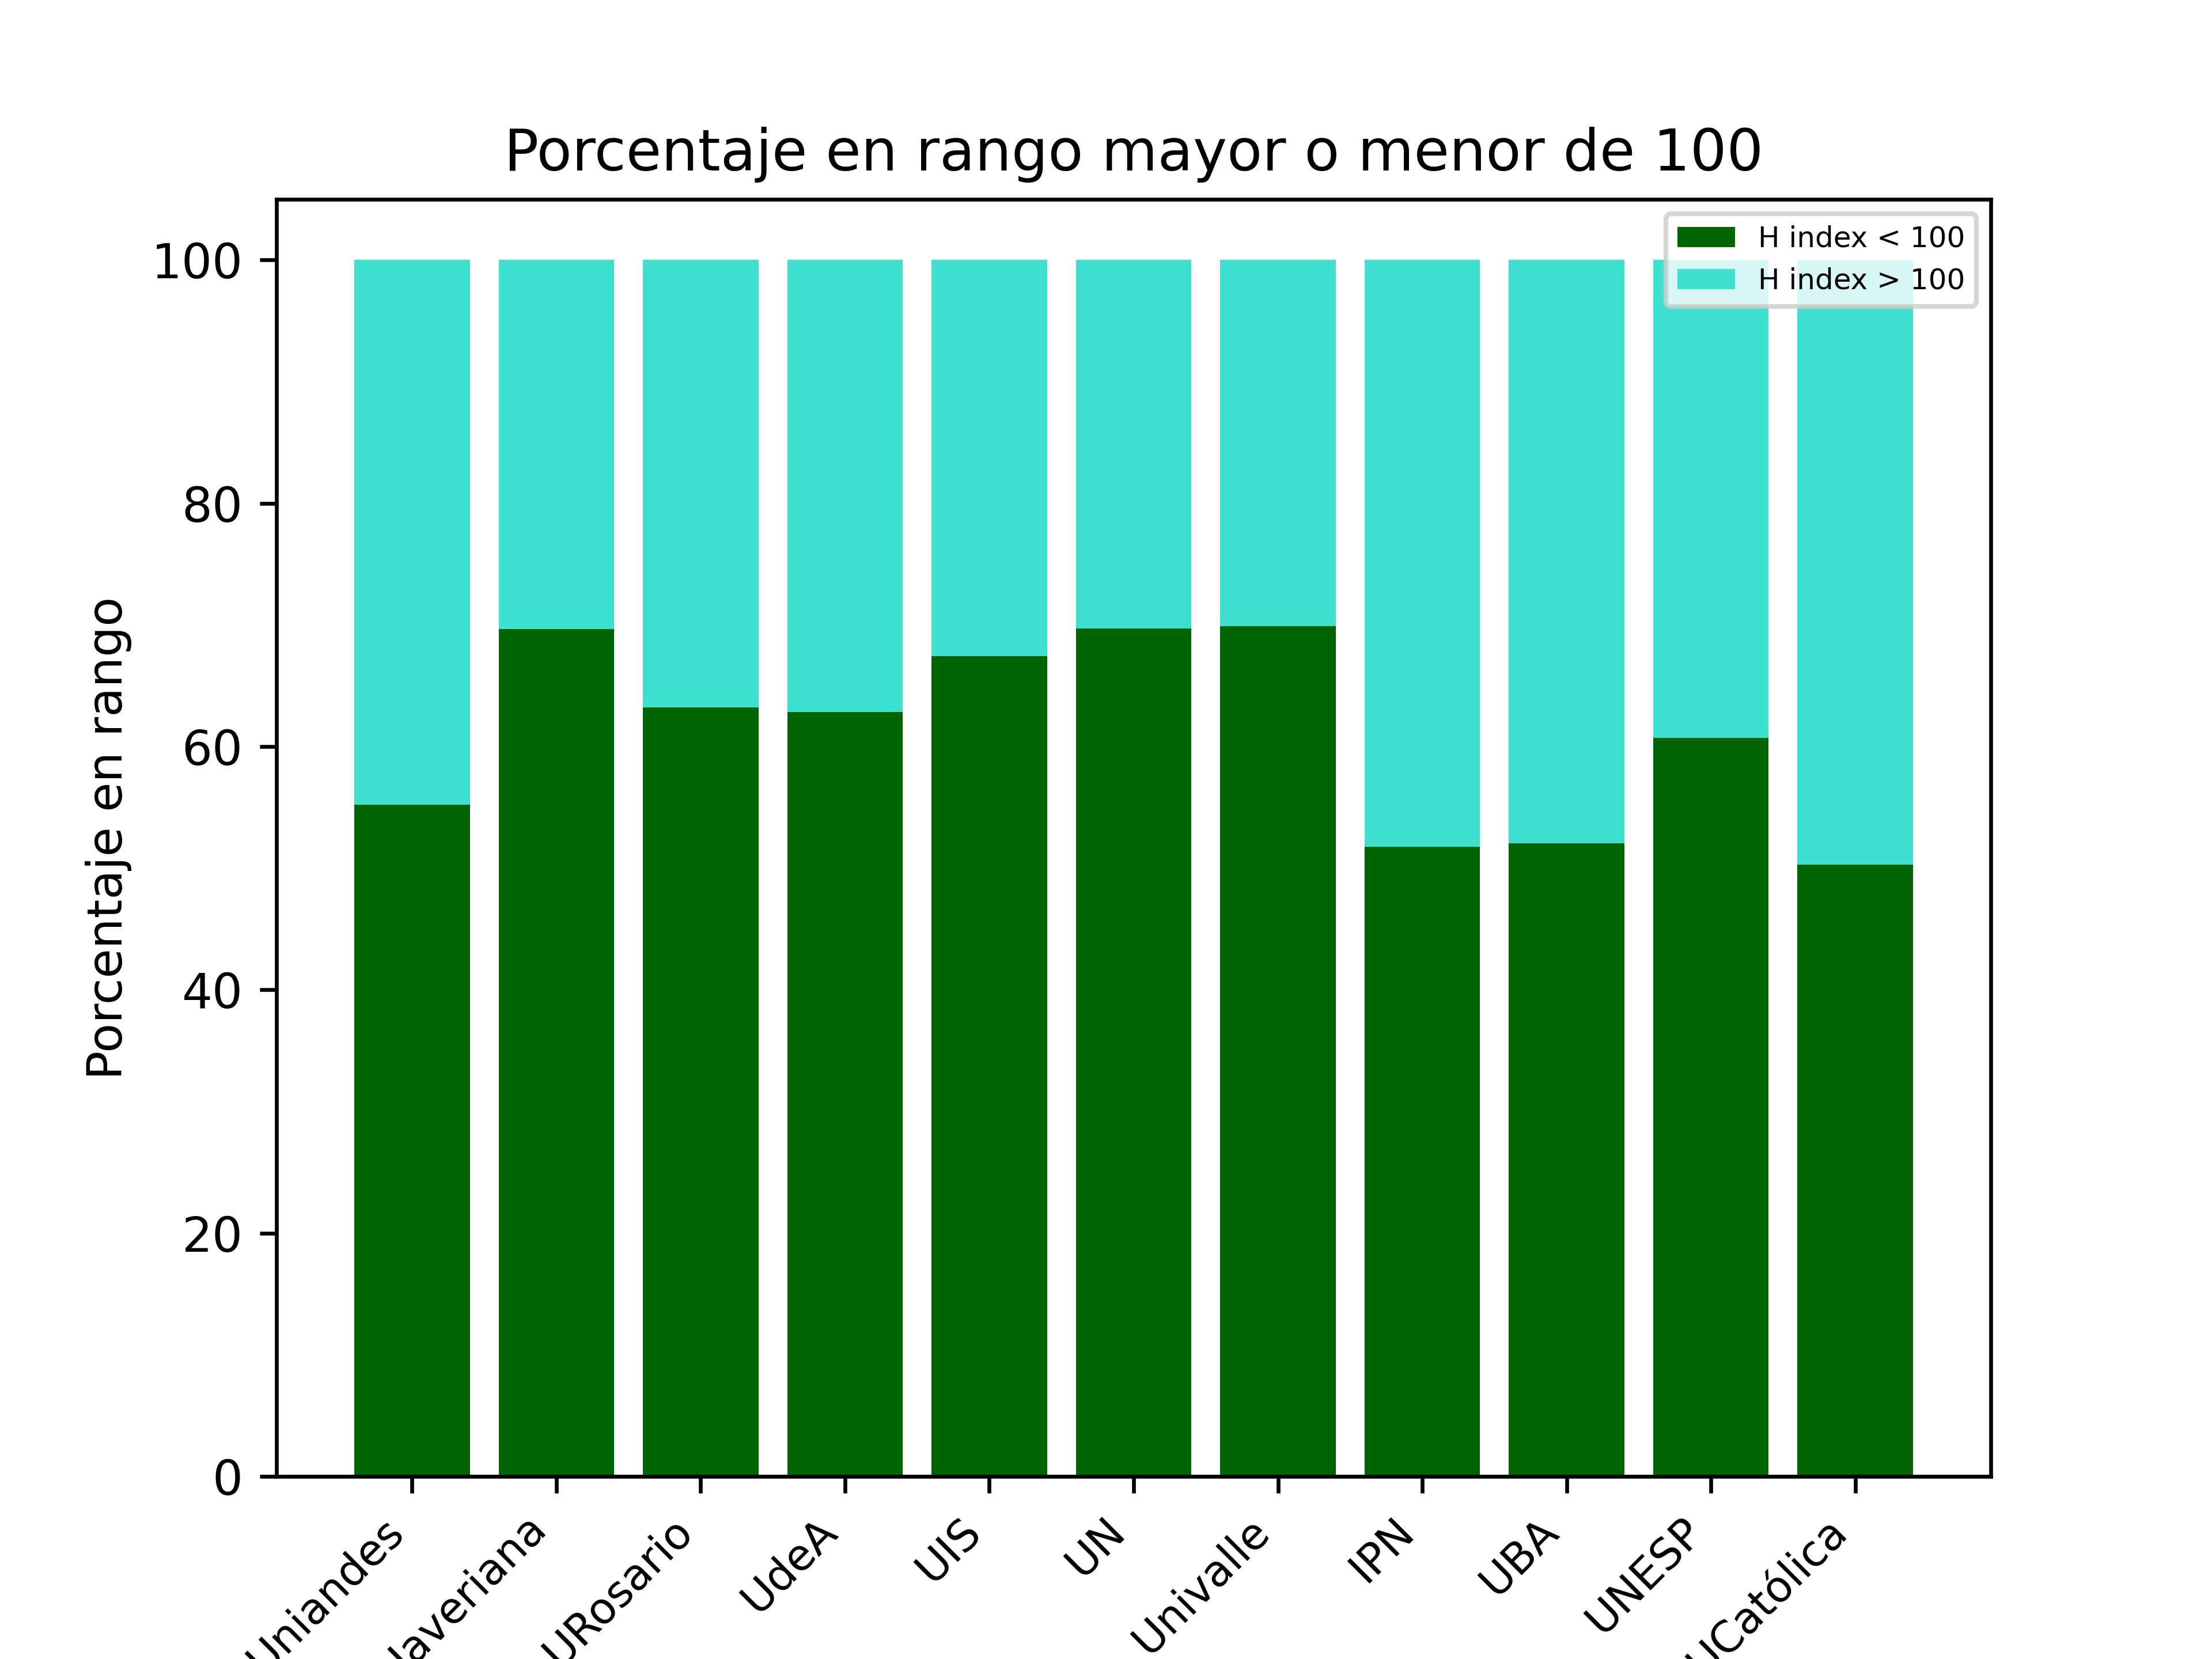
\includegraphics[width=67mm]{Porcentajes_mayor_menor_100_H.png}}
				{Selección según la producción \\ } 
			\end{tabular} \caption{\label{fig:porcentajeH}  Porcentaje de la producción en rangos de H-\textit{index} en el período 2013-2023.}
		\end{center}
	\end{figure}
\end{center} \vspace{-3mm}

\FloatBarrier

Es sí importante ese número al considerar la producción con los mejores H-\textit{index.} Esto por cuanto colaboraciones internacionales tienden a publicar en revistas de alto impacto (en el caso del CERN suelen ser revistas de un alto impacto). Una consulta a \cite{scimago-phys} y a \cite{inspire} muestra que las revistas usuales de las colaboraciones son Journal of High Energy Physics (H=247), Physical Review Letters (H=674), Physical Review D (H = 378), Physics Letters, section B (H= 275) y Europhysics letters (H=170). Con lo cual la fracción agregada como país a publicaciones de alto impacto se ve reducida según la tabla \ref{tab:cern}.

Un ruido imposible de filtrar completamente es la práctica de algunas instituciones de contratar personal de investigación en el exterior que en la práctica no está basado en Colombia. aunque aparece en las bases de datos como tal. Por asuntos de comunidades académicas fuertes las Instituciones seleccionadas se minimiza este riesgo. Es algo que existe en el sistema colombiano debido a la presión de tener investigación y acreditarla como sea para procesos con Minciencias o Mineducación y algunas IES toman atajos para mostrarla. 

Igualmente algunos investigadores adoptan la práctica de repetir las publicaciones en diferentes revistas. Esto es delicado pero suele afectar revistas de poco impacto así tomamos como que este ruido contribuye más al sector de publicaciones de bajos índicadores y no afecta las conclusiones en general.

Finalmente, no toda investigación o trabajo creativo es susceptible de publicaciones en revistas de alto impacto. Algunos trabajos son importantes solo a nivel local, por ejemplo, y no llevan necesariamente a publicaciones internacionales. Lo mismo sucede con producción tecnológica o aplicada. En este sentido este artículo se abstiene de hacer juicios al respecto y como es claro en título este trabajo es bibliométrico, debemos abstenernos de sacar conclusiones en otras dimensiones. 

\section{Conclusiones y recomendaciones.}

Se sientan bases y métodos para indagar y ahondar en la caracterización de la producción académica basada en investigación que se hace en Colombia, aunque sería de interés establecer una metodología que incluya otros tipos de producción académica. 

Los resultados dan evidencia de que se necesitan ajustes en la investigación en Colombia que incentiven la producción académica de alto impacto internacional (medido en número de citaciones y visibilidad) que nos lleven a los niveles al menos de las economías comparables de la región. Es indudable que para el Estado colombiano es costoso mantener la investigación que se hace y se deben buscar formas de mejorar los resultados de la investigación con los recursos disponibles o invertir recursos frescos con un propósito más estratégico.


\begin{thebibliography}{10}
	\bibitem{OpenAlex}
OpenAlex, \url{https://openalex.org/}, Ingreso en: 2024-03-07. 
	\bibitem{culbert} Reference Coverage Analysis of OpenAlex compared to Web of Science and Scopus.  
Jack Culbert, Anne Hobert, Najko Jahn, Nick Haupka, Marion Schmidt, Paul Donner and Philipp Mayr. 2024. \url{https://arxiv.org/abs/2401.16359v1}. 
	\bibitem{scimago} \url{https://www.scimagojr.com/aboutus.php}. Ingreso en: 2024-03-07.
	\bibitem{daemen} \url{https://libguides.daemen.edu/c.php?g=1239513&p=9072137}. 
	\bibitem{maryland} \url{https://lib.guides.umd.edu/bibliometrics/SJR}. Ingreso en: 2024-03-07.
	Ingreso en: 2024-03-07.
	\bibitem{western} \url{https://answers.library.westernsydney.edu.au/faq/269743}. 	Ingreso en: 2024-03-07.
	\bibitem{python}  Python Software Foundation. Python Language Reference. \url{https://python.org}
	\bibitem{jupyter} Kluyver, T.  Ragan-Kelley, B. Pérez, F. \textit{et. al.} ''Jupyter Notebooks -- a publishing format for reproducible computational workflows''.  Positioning and Power in Academic Publishing: Players, Agents and Agendas. IOS Press. 2016. pp. 87-90.
	\bibitem{mongo}   \url{https://www.mongodb.com/docs/manual/administration/install-on-linux/} Ingreso en 2024-03-20.
	\bibitem{ekolu} Ekolu, Stephen. ''Relationship between Research, Innovation and Development-a Review.'' EAI International Conference for Research, Innovation and Development for Africa. 2018.
	\bibitem{statista} https://www.statista.com/ Ingreso en 2024-03-20.
	\bibitem{luong}  Luong, H.M. Hewitt-Dundas, N. The interrelationship between R\&D, Innovation and Productivity:	Evidence for micro-enterprises.	Queen’s Management School and UK Enterprise 
	Research Centre. Apr. 2020. 
	\bibitem{celeste} Committee on Assessing the Value of Research in Advancing National Goals; Division of Behavioral and Social Sciences and Education; National Research Council; Celeste RF, Griswold A, Straf ML, editors. Furthering America's Research Enterprise. Washington (DC): National Academies Press (US); 2014 Oct 28. \url{https://www.ncbi.nlm.nih.gov/books/NBK253897/ doi: 10.17226/18804}
	\bibitem{scimago-phys} Revistas según su H-\textit{index.} \url{https://www.scimagojr.com/journalrank.php?order=h&ord=desc&area=3100#google_vignette} Accedida en 2024-03-22.
	\bibitem{inspire} Base de datos de publicaciones en física. \url{https://inspirehep.net/literature?sort=mostrecent&size=25&page=1&q=find%20collaboration%20cms} Accedida en 2024-03-22.
\end{thebibliography}

\newpage\section{Anexo técnico.} \label{sec:anexo}

Para el presente estudio se utiliza y es necesario disponer del siguiente software:
\begin{enumerate}
	\item Python 3, con bibliotecas numpy, matplotlib y panda \cite{python}.
	\item Jupyter notebooks \cite{jupyter}.
	\item Mongodb community edition, \cite{mongo}.
\end{enumerate}

El \textit{script}, los \textit{notebooks}, tablas, figuras y análisis están disponibles en \url{https://github.com/nvanegas/ImpactoDeInvestigaciones} excepto los archivos .csv que se crean. Estos deben ser bajados usando el \textit{script} que se provee para cada institución.

Las instrucciones para reproducir los resultados son:

\begin{enumerate}
	\item Copiar el repositorio de \textit{github} mencionado arriba. 
	\item Iniciar \textit{jupyter} y \textit{mongodb.}
	\item En cada subdirectorio (por institución) verificar el \textit{script} para bajar la información de OpenAlex que lleva la palabra \textit{download} en el nombre y verificar que en la tercera celda la ''I.D.'' de la institución de interés coincida con la dada en la tabla \ref*{tab:inst}.
	\item Ejecutar completo el \textit{notebook} de \textit{jupyter} de bajar información  (puede llevar algún tiempo). Esto debe repetirse para cada institución.
	\item Inmediatamente después entrar y ejecutar el \textit{notebook} de análisis en cada institución.  Los diccionarios de \textit{python} que resultan se llevan a tablas. Cada que se ejecuta uno de los \textit{notebooks} de bajar la información la base de datos cambia y no se debe mezclar el análisis de una universidad con la información bajada para otra.
	\item Verificar que la tabla dada en el repositorio de \textit{github} llamada ''nuevo-todos-3.csv'' coincide con los datos encontrados en el punto anterior. Es posible pequeñas diferencias pero no deben ser significativas.
	\item Ejecutar el \textit{notebook} de \textit{jupyter} llamado ''analisis-global-completo.ipynb'' y verificar tablas y gráficos.
\end{enumerate}





\end{document}